%% grundlagen.tex
%% $Id: grundlagen.tex 28 2007-01-18 16:31:32Z bless $
%%

\chapter{Background \& Related Work}
\label{ch:Background}

\section{Body Temperature}
In medical practice, temperature is one of the most frequently measured physical quantities.
By measuring temperature, one gains information about the internal energy of an object.
From the biophysical point of view, temperature measurement determines the changes in physical quantities that occur in a thermodynamic system. 
Temperature can be expressed in different scales.
These include Celsius, Fahrenheit, Kelvin, and Rankine \cite{grodzinskyUnderstandingFeverBody2020}.
When measuring body temperature, the skin temperature is often measured, which is then used to measure body temperature.
This is the result of a dynamic equilibrium between the heat released during metabolic processes and transferred to the skin layer by thermal conduction and convection, the heat extracted from the environment, and the heat transferred to the environment by radiation, convection, and evaporation.

\subsection{Thermal Regulation}
what is thermal regulation and why is it important
% TODO: fill with content

\subsection{Core Body Temperature}
Core body temperature is the temperature of the body's internal organs, such as the heart, liver, and brain, and is a commonly used indicator of human health and endurance performance.
Unlike the body core temperature, the body surface temperature is more easily influenced by the ambient temperature and therefore cannot reflect the changes inside the body as well as the body core temperature.
Core body temperature can be measured invasively rectally, orally (oesophagus), in the pulmonary artery (with the use of a catheter), or in the urinary bladder \cite{moranCoreTemperatureMeasurement2002a}. 
These types of measurements are uncomfortable for a person. 
In addition, because of this, it is not possible to take a measurement over a long period of time.

Body temperature can also be measured non-invasive.
This can be done on the axilla, the tympanic membrane, and the body surface \cite{moranCoreTemperatureMeasurement2002a}.

\subsection{Skin Temperature}
Pending content... 
% TODO: fill in with content

\subsection{Temperature Measurements}
% TODO: General Temperature measurements of human body
% Ear based temperature measeurements
Ear-based temperature measurement uses a sensor to measure the temperature of the ear canal. 
The approach has a number of advantages over other measurement positions.
First, it is a non-invasive measurement procedure, which allows measurement nearly inside the body with the least amount of hematoma.
Second, the measurement is much more promising compared to other non-invasive alternatives, where many factors can contribute to falsifying the final result \cite{ganioValidityReliabilityDevices2009, craigTemperatureMeasuredAxilla2000}. 
However, it is important to note that the accuracy of temperature measurement may depend on factors such as the positioning of the thermometer and the presence of earwax or other obstructions in the ear canal.

% \subsubsection{Temperature Measurements on the Tympanic Membrane}
The tympanic membrane is a thin membrane that separates the middle ear from the external auditory canal. 
The artery called the external carotid artery runs near the external auditory canal and radiates heat, which is why measuring the temperature at the tympanic membrane has a promising chance of determining body temperature \cite{yeohRevisitingTympanicMembrane2017}.

% TODO: \cite{yeohRevisitingTympanicMembrane2017} liefert in der introduction einiges zum thema blut temperatur und relevanz zu core body temperature

% TODO: \cite{ComparisonPulmonaryArtery}
% TODO: \cite{kimComparisonBilateralEardrum2022}
% TODO: \cite{childsTympanicMembraneTemperature1999}

\section{Temperature Sensors}
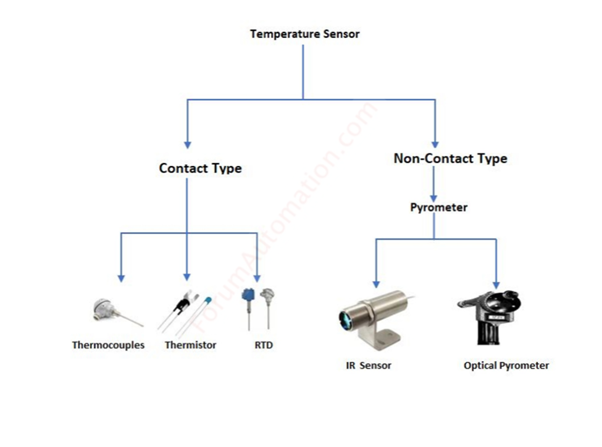
\includegraphics[scale=0.7]{thesis-doc/images/introduction/temp_sensor_types.png}

Temperature sensors are used to measure the temperature of a particular object or environment.
These are divided into 2 main categories, optical and thermal resistance sensors.
In this section, we will discuss the differences between these two types of sensors and their advantages and disadvantages.
% TODO: hier bisschen mehr auf die Grafik eingehen, die wird neu gebaut btw, verschwindet aber nicht
% Dann noch schreiben, auf was man genauer eingeht,


\subsection{Optical Temperature Sensors}
Optical temperature sensors measure the radiation emitted from an object at different wavelengths. 
This type of sensor is typically used in applications where contact with the object being measured is difficult or impossible, such as in space, harsh environments, or just where contact is not wanted.
Thus, non-contact measurements are possible, which is essential when measuring the temperature of the tympanic membrane.
Another advantage of optical temperature sensors is that moving objects can still be measured as long as the sensor continues to point at the object.
However, this requires a line of sight to the measured object.
In addition, accuracy can be affected by reflective surfaces or atmospheric conditions, which should not be a problem if the measurement is primarily in the ear.

\subsubsection{MLX}
% https://www.mouser.de/datasheet/2/734/MLX90632_Datasheet_Melexis-1595868.pdf

\subsection{Thermal Resistance Temperature Sensors}
Thermal resistance temperature sensors, also known as thermistors, operate by measuring changes in electrical resistance as a function of temperature. 
This type of sensor is typically used in applications where high accuracy is required, such as laboratory environments or medical equipment.
They provide high accuracy and cover a wide range of temperature measurements.
However, contact measurement is required here, which limits temperature measurement to stationary objects.
Furthermore, thermal resistance temperature sensors have a slow response time, which makes real-time measurement somewhat difficult.

In summary, optical temperature sensors are useful in situations where contact with the object being measured is difficult or impossible, while thermal resistance sensors are suitable for applications that require high accuracy and a wide temperature measurement range. 
Ultimately, the choice between these two types of sensors depends on the specific requirements of the application.

In the work applied here in the master's thesis, optical temperature sensors are suitable because they do not require direct contact points, which is essential when measuring temperature on the tympanic membrane.

\subsubsection{TPiS 1S 1385 / 5029}

\section{Sensing with Earables}
Earables belong to the class of wearables and are a type of wearable device that is worn in or around the ears. 
They typically have a number of sensors that allow them to collect data about the wearer's physiology and activity. 
The most common sensors in earables include accelerometers, gyroscopes, and heart rate monitors. These sensors can be used to track the wearer's movements, monitor their heart rate, and provide other types of health data.

% TODO: Now link the paper from Röddiger and extend with a summary of this paper
% 4 parts of sensing with earables
\subsection{Physiological Monitoring and Health}
\subsection{Movement and Activity}
\subsection{Interaction}
\subsection{Authentication and Identification}

\subsection{Sensing Platforms}
% TODO: Hier abschnitt zu sensing platforms, wie z.B OpenEarable






% https://media.digikey.com/pdf/Data%20Sheets/Excelitas%20PDFs/TPiS_1S_1385.pdf

% address translator weiter hinten, wo ich die implementierung ändere
% \subsection{Address translator}
% da die sensoren alle die gleiche addresse haben werden brauche wir da noch so address übersetzter, ich denke sopwas in die richung: 
% https://www.analog.com/media/en/technical-documentation/data-sheets/4316fa.pdf